\chapter{The computing Miniproject}
\label{chap:miniproj}

We have talked a lot about workflows and confronting models with data. 
It's time to do something concrete with all the techniques you have learnt!

The CMEE Miniproject gives you an opportunity to try the ``whole nine yards'' 
of developing and implementing a workflow and delivering a ``finished 
product'' --- where you ask and answer a scientific question in biology 
(potentially involving multiple sub-questions/hypotheses). 

The miniproject will give you an opportunity to perform a ``dry run'' 
of executing your actual dissertation project, and you may use it to 
trial some of the techniques and/or explore some of the data/theory  
you might use in your Dissertation project.

\section {Objectives}

{\bf The general question you will address is:} 

\begin{center}
	
\it What mathematical model best fits an empirical dataset?

\end{center}

You may think of this as testing a set of alternative hypotheses --- 
arguably every alternative hypothesis is nothing but an alternative model to 
describe an observed phenomenon (more on this in the Primer on Model 
Fitting Lectures delivered during the Miniproject week). 
 
You may choose any dataset and set of alternative models, provided that 
the work can feasibly be done in the time you have for your miniproject 
(see the CMEE Guidebook for the submission deadline). You may choose a 
problem and dataset that is a related to, or even preliminary work for 
your main Masters project (to give you a reality/feasibility) check.  

{\it Please read the papers in the Readings and Resources section of 
this chapter} --- these will help you make a decision about what data 
and what models to use.

You will also be give lectures on model fitting in Ecology ad Evolution 
at the start of the Miniproject week.  

The Miniproject must satisfy the following criteria:  
\begin{enumerate}
	
	\item It should employ all the biological computing tools you 
	have learned so far: shell (bash) scripting, git, \LaTeX, R, and 
	Python. Using these tools, you will build a workflow that starts with 
	the data and ends with a written report (in \LaTeX).
	
	\item {\it At least} two different models (hypotheses) must be fitted 
	to the data. The models should be fitted and selected using an 
	appropriate method (e.g., non-linear least squares for model fitting and 
	the Akaike Information Criterion for model selection, respectively). 
	You will be given a primer on model fitting before you start on your 
	Miniproject. 
	
	\item The project should be fully reproducible --- a script should 
	glue the workflow together and run it. I should be able to run just 
	this script to get everything to work, from data processing to model 
	fitting to plotting (e.g., in {\tt R}) to compilation of the \LaTeX 
	written report. ({\it More detailed instructions on this below}). 
	   
\end{enumerate}

If you are unable to find a dataset and/or problem that you would like 
to tackle, you may use the ``TPC problem'' given below.

\section{The Report}

	The report should,
	\begin{compactitem}
		\item be written in \LaTeX~ using the {\tt article} document class, 
		in 11pt (any font will do, within reason!)
	
		\item be double-spaced, with {\it continuous} line numbers 
	
		\item have a title, author name with affiliation and wordcount 
		(next point) on a separate title page.
		
		\item have an introduction with objectives of the study, and 
		appropriate additional sections such as methods, data, results, 
		discussion, etc. 
		\item should contain in the Methods a sub-section called 
		``Computing languages'' which states briefly how each of the three 
		scripting language (bash, R, Python) was used, and a justification 
		of why. 
		\item must contain $\leq$3500 words {\it excluding the contents of 
		the title page, references, and Figure or Table captions+legends}; 
		there should be a word count at the beginning of the document (I 
		suggest using {\tt texcount}).
	
		\item have references properly cited using bibtex.
	
	\end{compactitem}

For the writeup, you probably should read the {\it general} ( {\it 
not} word count, formatting etc.) dissertation writing guidelines given 
in the Silwood Masters Student Guidebook.  

\section{Patching together your computing workflow components}

Use Python and/or bash scripting for this. If using bash, call it  {\tt 
run\_MiniProject.sh} and if using Python, called it {\tt 
run\_MiniProject.py}. It should run all the components of the project's 
workflow, including compilation of the \LaTeX document. Look back at 
the notes to see how you would run these different components. For 
example, we have covered how to run {\tt R} and compile \LaTeX using {\tt 
subprocess} in python.

\section{Submission}

Commit and push all your work to your bitbucket repository using a 
directory called {\tt CMEEMiniProject} at the same level as the {\tt 
Week1}, {\tt Week2} etc. directories, by the Miniproject deadline given 
in your CMEE course guidebook.

At this stage, I am not going to tell you how to organize your project 
--- that's one of my marking criteria (see next section). 

\subsection {Marking criteria}

{\it Equal weightage will be given to the code+workflow and writeup 
components --- each component will be marked to a max of 100 pts and 
then rescaled to a single mark / 100 using equal weightage}
 
I will be looking for the following while assessing your submission:

\begin{compactitem}

	\item A well-organized project where code, results, data, etc., are 
	easy to locate, inspect, and use. In the project's README also 
	include: 
	\begin{itemize}
	\item Any dependencies or special packages I should be aware of  	
	\item What each package you used is for
	\item Version of each language used
	\end{itemize}

	\item A python or bash script called {\tt run\_MiniProject.py} or {\tt 
	run\_MiniProject.sh} respectively, that runs the project

	\item A report that contains all the components indicated above in 
	``The Report'' subsection --- I will be looking for some original 
	thought and synthesis in the Intro and Discussion

	\item Quality of the presentation of the graphics and tables in your 
	report, as well as any plots showing model fits to the data.  

\end{compactitem}

The marking criteria you may refer to is the summative marking criteria 
given in Appendix \ref{chap:Appendices} titled ``MARKING CRITERIA for 
EXAMS and ESSAYS and COURSEWORK''.  

\section {A Candidate Problem: Fitting TPCs}

One choice you have is to use a large dataset that we can provide to 
address the following question: 

{\it How well do different mathematical models, based upon biochemical 
principles vs. phenomenological ones, fit to the thermal responses of 
metabolic traits (rates)?}

This is currently a ``hot'' (no pun intended!) topic in biology, with 
both ecological and evolutionary consequences, as we discussed in the 
modelling lecture. On the {\it ecological side}, because the 
temperature-dependence of metabolic rate sets the rate of intrinsic 
$r_{max}$ (papers by Savage et al., Brown et al.) as well as 
interactions between species, it has a strong effect on population 
dynamics. In this context, note that 99.9\% of life on earth is 
ectothermic! On the {\it evolutionary side}, the temperature-dependence 
of fitness and species interactions also means that warmer environments 
may have stronger rates of evolution. This may be compounded by the 
fact that mutation rates may also increase with temperature (papers by 
Gillooly et al.).

\subsection{The Data}

The dataset is called {\tt BiotraiTPCdata.csv} and contains hundreds of 
``thermal responses'' for growth, respiration and photosynthesis rates 
in plants and bacteria (both aquatic and terrestrial). These data were 
collected through lab experiments across the world, and compiled by 
various people over the years. A subset of this BioTraits database used 
as an example in the Databases section of Chapter \ref{chap:pythonII}.

\subsection {The Models}

There are multiple models that might best describe these data.

The Schoolfield model (paper is in {\tt Readings} directory) is one
mechanistic option (\ref{fig:schoolf}) that is based upon 
thermodynamics and enzyme kinetics:

\begin{equation} \label{eq:schoolf}
	\begin{aligned}
	  B = \frac{B_0 e^{\frac{-E}{k} (\frac{1}{T} - \frac{1}{283.15})}}
    { 1 + e^{\frac{E_l}{k} (\frac{1}{T_l} - \frac{1}{T})} + 
    e^{\frac{E_h}{k} (\frac{1}{T_h} - \frac{1}{T})}}
	\end{aligned}
\end{equation}

{\it Please also have a look at the Delong et al 2017 paper, which lists 
this and other mechanistic TPC models} (see the Readings and 
Resources section). Youy may choose additional models listed in that 
paper for comparison, if you want.

Here, $k$ is the Boltzmann constant ($8.617 \times 10^{-5}$ eV $\cdot$ 
K$^{-1}$), $B$ the value of the trait at a given temperature $T$ (K) (K 
= $\degree$C + 273.15), while $B_0$  is the trait value at 283.15 K 
(10\degree C) which stands for the value of the  growth rate at low 
temperature and controls the vertical offset of the curve. $E_l$ is the 
enzyme's low-temperature de-activation energy (eV) which controls the 
behavior of the enzyme (and the curve) at very low temperatures, and 
$T_l$ is the at which the enzyme is  50\% low-temperature deactivated. 
$E_h$ is the enzyme's high-temperature de-activation energy (eV) which 
controls the behavior of the enzyme (and the curve) at very high 
temperatures, and $T_h$ is the at which the enzyme is  50\% 
high-temperature deactivated. $E$ is  the activation energy (eV) which 
controls the rise of the curve up to the peak in the ``normal operating 
range'' for the enzyme (below the peak of the curve and above $T_h$). 

\begin{figure}\label{fig:schoolf}
		\centering 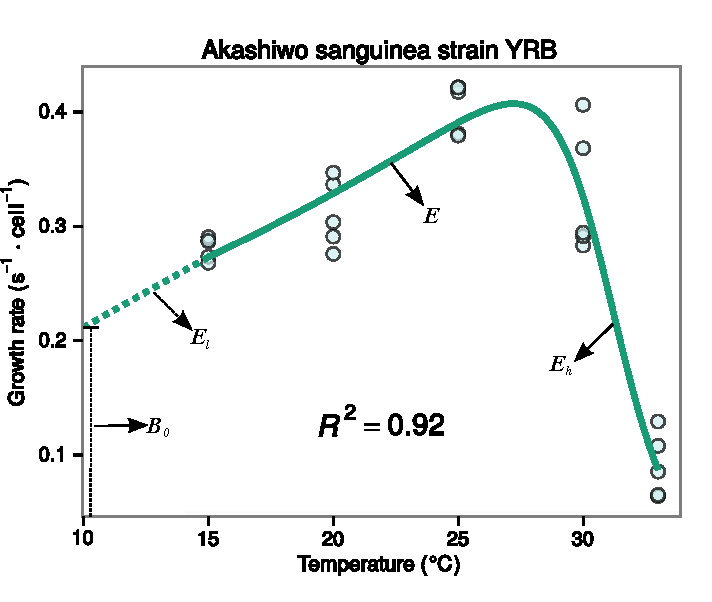
\includegraphics[width=.6\textwidth]{SchoolfEx.pdf} 
		\caption{Example of a unimodal thermal response curve for a 
		biological trait with the Schoolfield model fitted (Equation 
		\ref{eq:schoolf}).}
\end{figure}

In many cases, a simplified Schoolfield model would be more appropriate 
for thermal response data, because low temperature inactivation is 
weak, or is undetectable in the data because low-temperature 
measurements were not made.

\begin{equation} \label{eq:schoolfHi}
	\begin{aligned}
	  B = \frac{B_0 e^{\frac{-E}{k} (\frac{1}{T} - \frac{1}{283.15})}}
    { 1 +  e^{\frac{E_h}{k} (\frac{1}{T_h} - \frac{1}{T})}}
	\end{aligned}
\end{equation}

In other cases, a different simplified Schoolfield model would be more 
appropriate, because high temperature inactivation was not detectable 
in the data because measurements were not made at sufficiently high 
temperatures:

\begin{equation} \label{eq:schoolfLo}
	\begin{aligned}
	  B = \frac{B_0 e^{\frac{-E}{k} (\frac{1}{T} - \frac{1}{283.15})}}
    { 1 +  e^{\frac{E_l}{k} (\frac{1}{T_l} - \frac{1}{T})}}
	\end{aligned}
\end{equation}

In addition, there are phenomenological alternatives. These include the 
general cubic polynomial model:

\begin{equation}\label{eq:cubic}
	B = B_0 + B_1 T + B_2 T^2 + B_3 T^3
\end{equation}
with the parameters $B_0$, $B_1$, $B_2$ and $B_3$ not having any 
mechanistic underpinnings. Note that the cubic model has the same 
number of parameters as the the reduced Schoolfield model 
\ref{eq:schoolfH}. The parameter ($T$) of the cubic model (Equation 
\ref{eq:cubic}) are in $\degree$C.

{\it All the above parameters and equations are in SI units}.

\subsection {Fitting models to the TPC data}

You will use Nonlinear Least Squares (NLLS) to fit the alternative 
models above (eqns \ref{eq:schoolf} -- \ref{eq:cubic}) to data, 
followed by model selection with AIC and BIC (also known as the 
Schwartz Criterion --- {\it read the Johnson and Omland 2005 paper}).
 
\subsection {The Workflow}

You will build a workflow that starts with the data and ends with a 
report written in \LaTeX. I suggest the following components and 
sequence in your workflow (you can choose to do it differently!):

\begin{enumerate}\itemsep0pt
	\item A Python or R script that imports the data and prepares it for 
	NLLS fitting, with the following features:
		\begin{compactitem}
			\item It should create unique ids so that you can identify unique 
			thermal responses (what does this mean?) 
			\item It should filter out datasets with less than 5 data points 
			(why?)
			\item It should deal with negative and zero trait values (why?) 
			\item The script should add columns containing starting values 
			of the model parameters for the NLLS fitting (how will you get 
			these?)
			\item Save the modified data to a new csv file. 
		\end{compactitem}
	\item A Python script that opens the new modified dataset (from 
	step 1) and does the NLLS fitting, with the following features:
			\begin{compactitem}
				\item Uses {\tt lmfit} --- look up submodules {\tt minimize}, 
				{\tt Parameters}, {\tt Parameter}, and {\tt report\_fit}.\\
				{\it Have a look through} 
				\url{http://lmfit.github.io/lmfit-py}, especially 
				\url{http://lmfit.github.io/lmfit-py/fitting.html#minimize}\\
				
				You will have to install lmfit using {\tt pip} or {\tt 
				easy\_install} - use {\tt sudo} mode.
				In addition to the lmfit example in class, you may want to look 
				for others online.
				
				\item Will use the {\tt try} construct because not all runs 
				will converge. Recall the {\tt try} example from R

				\item The more thermal response curves you are able to fit, the 
						better --- that is part of the challenge!

				\item Will calculate AIC, BIC, R$^{2}$, and other statistical 
				measures of fit (you decide what you want to include)
				
				\item Will export the results to a csv that the plotting R 
				script (next item) can read.

		\end{compactitem}

	\item A {\tt R} script that imports the results from the previous 
	step and plots every thermal response with both models (or none, if 
	nothing converges) overlaid --- all plots should be saved in a 
	single separate sub-directory. {\it Use {\tt ggplot} for pretty 
	results!} 

	\item \LaTeX~source code that generates your report.
	
	\item A Python script (saved in {\tt Code}) called {\tt 
	run\_MiniProject.py} that runs the whole project, right down to 
	compilation of the \LaTeX~ document. 

\end{enumerate}

Doing all this may seem a bit scary at the start. However, you need to 
approach the problem systematically and methodically, and you will be 
OK. I suggest the following to get you started:

\begin{compactitem}

	\item Explore the data in R and get a preliminary version of the 
	plotting script without the fitted models overlaid worked out. That 
	will also give you a feel for the data.

	\item Explore the two models -- be able to plot them. Write them as 
	functions in your {\tt python} script, because that's where you 
	will use them (step 2 above) (you can use {\tt matplotlib} for 
	quick and dirty plotting and then suppress those code lines later).

	\item Figure out, using a minimal example (say, with one, 
	"nice-looking" thermal response dataset) to see how the {\tt python}
	{\tt lmfit} module works. Kartik can help you work out the minimal
	example, including the usage of {\tt try} to catch errors in case the
	fitting doesn't converge. 
	
	\item One thing to note is that you will need to do the NLLS fitting 
	on the logarithm of the the function to facilitate convergence --- 
	please ask me or Sam Thompson if you need help on this.
	
\end{compactitem}

\section{Readings and Resources}

All these papers are in pdf format in the {\tt Readings} directory on the CMEE master repository. 

\begin{compactitem} \itemsep6pt
\item Levins, R. (1966) The strategy of model building in population 
biology. Am. Sci. 54, 421--431.  

\item Johnson, J. B. \& Omland, K. S. (2004) Model selection in ecology 
and evolution. Trends Ecol. Evol. 19, 101--108. 

\item Bolker, B. M. et al.  (2013) Strategies for fitting nonlinear ecological models in R, AD Model Builder, and BUGS. Methods Ecol. Evol. 4, 501--512 .

\item Some illustrative examples of (nonlinear) model-fitting to 
ecological/evolutionary data 
\url{https://groups.nceas.ucsb.edu/non-linear-modeling/projects} 

\item For the suggested fitting TPCs project: Papers in the {\tt 
Temperature\_response\_papers} directory within , but especially : 


\begin{itemize}
	
\item Schoolfield, R. M., Sharpe, P. J. \& Magnuson, C. E. (1981) Non-linear 
regression of biological temperature-dependent rate models based on 
absolute reaction-rate theory. J. Theor. Biol. 88, 719--31. 

\item DeLong, J. P. et al. (2017) The combined effects of reactant kinetics and enzyme stability explain the temperature dependence of metabolic rates. Ecol. Evol. 7, 3940--3950 .

\end{itemize}

\end{compactitem}
